\subsection{春节}
\par
春节,即农历新年,是一年之岁首,亦为传统意义上的“年节”。俗称新春、新岁、新年、新禧、年禧、大年等,口头上又称度岁、庆岁、过年、过大年。春节历史悠久,由上古时代岁首祈年祭祀演变而来。万物本乎天、人本乎祖,祈年祭祀、敬天法祖,报本反始也。春节的起源蕴含着深邃的文化内涵,在传承发展中承载了丰厚的历史文化底蕴。在春节期间,全国各地均有举行各种庆贺新春活动,热闹喜庆的气氛洋溢;这些活动以除旧布新、迎禧接福、拜神祭祖、祈求丰年为主要内容,形式丰富多彩,带有浓郁的各地域特色,凝聚着中华传统文化精华。
在现代,人们把春节定于农历正月初一,但一般至少要到农历正月十五(元宵节)新年才算结束。春节是个欢乐祥和、亲朋好友欢聚的节日,是人们增深感情的纽带。节日交流问候传递着亲朋乡里之间的亲情伦理,它是维系春节得以持存发展的重要要义。
\par
百节年为首,春节是中华民族最隆重的传统佳节,它不仅集中体现了中华民族的思想信仰、理想愿望、生活娱乐和文化心理,而且还是祈福、饮食和娱乐活动的狂欢式展示。受到中华文化的影响,世界上一些国家和地区也有庆贺新春的习俗。据不完全统计,已有近20个国家和地区把中国春节定为整体或者所辖部分城市的法定节假日。春节与清明节、端午节、中秋节并称为中国四大传统节日。春节民俗经国务院批准列入第一批国家级非物质文化遗产名录。   
\par
年节是中国一个古老的节日,也是全年最重要的一个节日,在历史发展中,杂糅了多地多种民俗为一体,形成了一些较为固定的风俗习惯,有许多还相传至今。中国是个多民族的国家,各民族过新年的形式各有不同。春节是汉族最重要的节日,满、蒙古,瑶、壮、白、高山、赫哲、哈尼、达斡尔、侗、黎等十几个少数民族也有过春节的习俗,只是过节的形式更有自己的民族特色,更蕴味无穷。春节期间的庆祝活动极为丰富多样,有舞狮、飘色、舞龙、游神、庙会、逛花街、赏花灯、游锣鼓、游标旗、烧烟花、祈福、掼春,也有踩高跷、跑旱船、扭秧歌等等。祭祀神(祖)习俗盛行于南方沿海一带,承袭古时习俗,春节期间多地有举行隆重盛大的报祭天地神恩、迎禧祈福等祭祝祈年活动,内容丰富多彩,热闹喜庆,年味浓郁。春节期间贴年红、守岁、吃团年饭、拜年等各地皆有之,但因风土人情的不同,细微处又各有其特色。春节民俗形式多样、内容丰富,是中华民族的生活文化精粹的集中展示。
\par
春节是除旧布新的日子,春节虽定在农历正月初一,但春节的活动却并不止于正月初一这一天。从年尾廿三(或廿四日)小年起,人们便开始“忙年”:祭灶、扫尘、购置年货、贴年红、洗头沐浴、张灯结彩等等,所有这些活动,有一个共同的主题,即“辞旧迎新”。春节是个欢乐祥和、合家团圆的节日,也是人们抒发对幸福和自由向往的狂欢节和永远的精神支柱。过节前,别井离乡的人们都尽可能地回到家里和亲人团聚,共享天伦之乐。除夕,全家欢聚一堂,吃罢“团年饭”,长辈给孩子们派发“压岁钱”,然后“守岁”,迎接新年到来。年节期间,亲朋好友之间相互走访拜年,表达对亲朋好友之间的情怀以及对新一年生活的美好祝愿。
春节也是敦亲祀祖、祭祝祈年的日子。在热闹非常的春节期间,敬天法祖传统文化祭祀节仪才依循祖上规矩,进贡上香,叩拜行礼,庄重肃穆,一丝不苟。

\begin{figure}[htb]
    \centering 
    \begin{subfigure}[t]{0.48\linewidth}
    \centering
    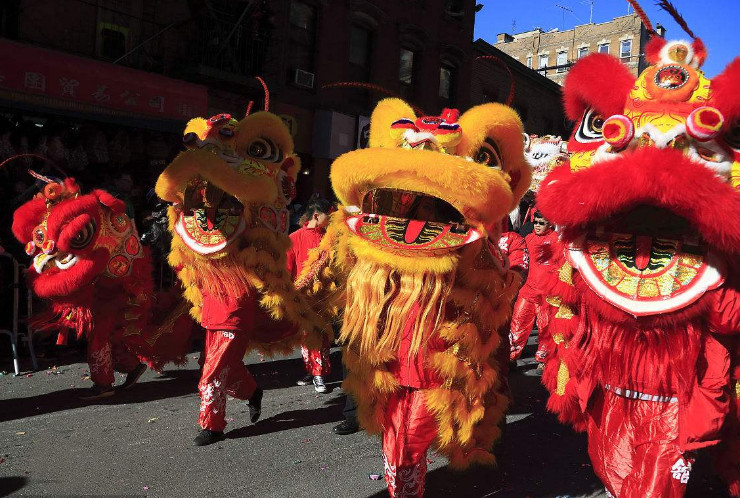
\includegraphics[width=\linewidth]{wushi}
    \caption{舞狮}        
    \end{subfigure}
    \begin{subfigure}[t]{0.48\linewidth}
        \centering
    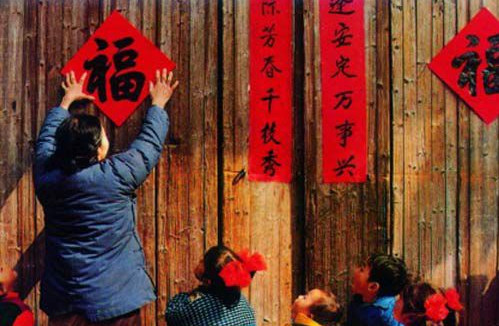
\includegraphics[width=\linewidth]{tienianhong}
    \caption{贴年红}        
    \end{subfigure}

    \begin{subfigure}[t]{0.48\linewidth}
        \centering
    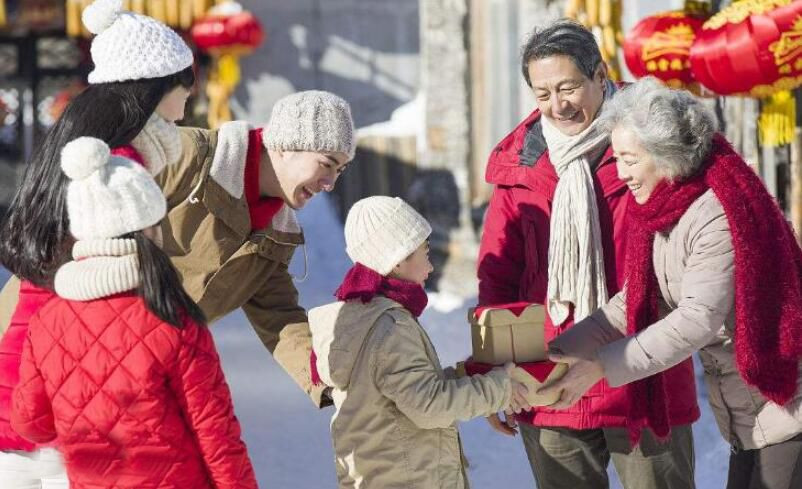
\includegraphics[width=\linewidth]{besuchen}
    \caption{拜年}        
    \end{subfigure}
    \begin{subfigure}[t]{0.48\linewidth}
        \centering
    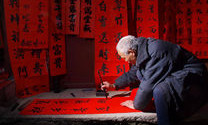
\includegraphics[width=\linewidth]{chunlian}
    \caption{写春联}        
    \end{subfigure}
    \caption{春节习俗} 
\end{figure}
\subsubsection{习俗}

\begin{enumerate}
    
\item \textbf{办年货}

中国的年俗文化源远流长,全国各地衍生出纷繁多样的过年习俗,南北迥异,各具特色。虽然各地习俗不尽相同,但是备年货、送年礼却是几乎全国上下的“过年必备”。置办年货,包括吃的、穿的、戴的、用的、贴的(年红)、送的(拜年)礼物等等,统名曰之“年货”,而把采购年货的过程称之为“办年货”。办年货是中国人过春节的一项重要活动。

\item \textbf{祭灶}

农历十二月廿三/廿四日祭灶,是日入夜后要把灶台刷干净,把旧的灶君神像取下烧掉,除至夕日晨早把新像贴上,一送一迎,都要摆置酒肉、糖果、甘蔗、米果等,烧香、点烛、放纸炮。民间祭灶,源于古人拜火习俗。《释名》:“灶。造也,创食物也。”灶神的职责就是执掌灶火,管理饮食,后来扩大为考察人间善恶,以降福祸。祭灶在中国民间有几千年历史了,灶神信仰是中国百姓对“衣食有余”梦想追求的反映。

\item  \textbf{扫尘}

在民间,新年前夕有“腊月二十四,扫尘(亦称扫屋)的习俗 。民谚称“二十四,扫房子”。民间称做“扫尘日”。扫尘就是年终大扫除, 家家户户都要打扫环境,清洗各种器具,拆洗被褥窗帘,洒扫六闾庭院,掸拂尘垢蛛网,疏浚明渠暗沟。到处洋溢着欢欢喜喜搞卫生、干干净净迎新春的欢乐气氛。按民间的说法:因“尘”与“陈”谐音,年前扫尘有“除陈布新”的涵义。扫尘用意是要把一切穷运、晦气统统扫出门,以祈来年清吉。

\item \textbf{贴年红}

年廿八、廿九或三十日家家户户“贴年红”(年红是春联、门神、横批、年画、“福”字等过年时所贴的红色喜庆元素统称)。过年贴年红(挥春),是中国传统的过年习俗,增添了喜庆的节日气氛,并寄予着人们对新年和新生活的美好期盼。

\item \textbf{年夜饭}

年夜饭,又称年晚饭、团年饭、团圆饭等,特指岁末除夕的阖家聚餐。年夜饭源于古代的年终祭祀仪,拜祭神灵与祖先后团圆聚餐。年夜饭是年前的重头戏,不但丰富多彩,而且很讲究意头。吃团年饭前先拜神祭祖,待拜祭仪式完毕后才开饭。席上一般有鸡(寓意有计)、鱼(寓意年年有余)、蚝豉(寓意好市)、发菜(寓意发财)、腐竹(寓意富足)、莲藕(寓意聪明)、生菜(寓意生财)、生蒜(寓意会计算)、腊肠(寓意长久)等以求吉利。中国人的年夜饭是家人的团圆聚餐,这顿是年尾最丰盛、最重要的一顿晚餐。

\item \textbf{守岁}

除夕守岁是年俗活动之一,守岁之俗由来已久。守岁的民俗主要表现为所有房子都点燃岁火,合家欢聚,并守“岁火”不让熄灭,等着辞旧迎新的时刻,迎接新岁到来。除夕夜灯火通宵不灭,曰“燃灯照岁”或“点岁火”,所有房子都点上灯烛,还要专门在床底点灯烛,遍燃灯烛,谓之“照虚耗”,据说如此照过之后,就会使来年家中财富充实。古时南北风俗各异,古时北方一些地方守岁习俗主要为熬年夜,如晋朝周处所著的《风土记》中说:除夕之夜大家各相与赠送,称“馈岁”;长幼聚欢,祝颂完备,称“分岁”;终岁不眠,以待天明,称“守岁”。除夕之夜,全家团聚在一起,吃过年夜饭,点起蜡烛或油灯,围坐炉旁闲聊,通宵守夜,象征着把一切邪瘟病疫照跑驱走,期待着新的一年吉祥如意。

\item \textbf{压岁钱}

压岁钱,年俗之一,年晚饭后长辈要将事先准备好的压岁钱派发给晚辈,据说压岁钱可以压住邪祟,晚辈得到压岁钱就可以平平安安度过一岁。压岁钱在民俗文化中寓意辟邪驱鬼,保佑平安。压岁钱最初的用意是镇恶驱邪。因为人们认为小孩容易受鬼祟的侵害,所以用压岁钱压祟驱邪。

\item \textbf{游神}

传统贺岁习俗之一,游神,又称圣驾巡游、游老爷、营老爷、游菩萨、游神赛会、年例、迎神、迎年、游春、行香、菩萨行乡、抬神像、神像出巡等等,是指人们在新年期间或其它喜庆节日里,又或诸神圣诞的这一天,到神庙里将行身神像请进神轿里,然后抬出庙宇游境,接受民众的香火膜拜,寓意神明降落民间,巡视乡里,保佑合境平安。主旨是酬神、消灾、祈福等。游神沿途伴随有锣鼓、唢呐、神偶、舞狮、舞龙、飘色、标旗、游灯、八音、杂技及乐队演奏等丰富多彩艺阵表演。是集拜神、祈祷、欢庆、宴客为一体的传统民俗活动。

\item \textbf{拜岁}

拜岁,年俗活动之一。在岁首早上迎新岁,拜祭“岁神”。“岁”又名为“摄提”、“太岁”,上古纪元星名。太岁也是民间信仰的神灵。岁以六十甲子的干支纪年法为运转周期,共六十位,每年有一位岁神当值,在当年当值的太岁谓之“值年太岁”,是一岁之主宰,掌管当年人间的吉凶祸福。如《三命通会》中所讲:“夫太岁者,乃一岁之主宰,诸神之领袖”。拜岁是历史最悠久的过年传统风俗,这古俗如今在广东,尤其在吴川一带仍盛行。在新年初一辞旧迎新之际,迎新岁、拜祭岁神、接福,这一传统习俗自古以来代代相传。

\item \textbf{庙会}

逛庙会是春节期间的民俗活动之一。广府庙会与北京地坛庙会并称中国两大庙会。涵盖木偶荟萃、中华绝活、武林大会、元宵灯会等主题活动,包含了祈福文化、民俗文化、美食文化、商贸休闲文化等丰富的内容。

\item \textbf{拜年}

春节期间走访拜年是年节传统习俗之一,是人们辞旧迎新、相互表达美好祝愿的一种方式。初二、三就开始走亲戚看朋友,相互拜年,道贺祝福,说些恭贺新喜、恭喜发财、恭喜、新年好等话。拜年的意义所在是亲朋好友之间走访联络感情、互贺新年,表达对亲朋间的情怀以及对新一年生活的美好祝福。

\item \textbf{派利是}

派利是,是流传已久的年俗之一,“利是”亦有写作“利市”或“利事”。派利是,利是利是,寓意着一年都能利利是是,大红大紫。“利市”一词古已有之,早在《易经》中便有记载,带有本少利多的意思。元代《俗谚考》亦提及“为了吉兆,要向主家讨个利市”的说法,由此可见,利市亦有好运的意义。 根据《易杂注》所载:“营商利市,营达利事”,生意人派的叫利市,取其有利于做任何事情的意思。

\item \textbf{烧炮竹}

中国民间有“开门炮仗”一说。即在新的一年到来之际,家家户户开门的第一件事就是烧炮竹,以哔哔叭叭的爆竹声除旧迎新。炮竹是中国特产,亦称“爆仗”、“爆竹”、“炮仗”、“鞭炮”。其起源很早,关于爆竹的演变过程,《通俗编排优》记载道:“古时爆竹。皆以真竹着火爆之,故唐人诗亦称爆竿。后人卷纸为之。称曰“爆竹”。
炮竹的原始目的是迎神与驱逐鬼怪。后来以其强烈的喜庆色彩发展为辞旧迎新的象征符号。烧炮竹可以创造出喜庆热闹的气氛,是节日的一种娱乐活动,可以给人们带来欢愉和吉利。

\item \textbf{春晚}

春节联欢晚会,通常简称“春晚”,是中国中央电视台在每年除夕晚上为庆祝农历新年举办的综艺性文艺晚会。1983年,央视举办春节联欢晚会应该说是一个偶然事件。但是这台晚会已经成为了中国人的“新民俗,新文化”,每年除夕夜必看的电视大餐。从1983年起,央视春晚这枚凝聚了十几亿中国人亲情与乡愁的符号,已经成为几代中国人的文化记忆。 [114] 
从文化发展的角度看,中央电视台春节联欢晚会开创了电视综艺节目的先河,且引发了中国电视传媒表达内容、表达方式等方面的重大变革。春节联欢晚会涵盖小品、歌曲、歌舞、杂技、魔术、戏曲、相声剧等多种表演形式。

\end{enumerate}

\subsubsection{中国春运}
\par
春节期间的运输,简称为”春运“。是中国特有的一种运输期间。以春节为界,节前15天,节后25天,共40天,由国家经贸委统一发布(每年起止时间略有不同),铁道部、交通部、民航总局按此进行专门运输安排的全国性交通运输高峰叫做春运。
\par
春运期间,铁道部实行特殊运行管理,加开大量临时客车,时间为春节前后15天。80年代以后,大量民工外出,春运成为社会热点。
\par
“春运”被誉为人类历史上规模最大的、周期性的人类大迁徙。在40天左右的时间里,将有20多亿人次的人口流动,占世界人口的1/3。中国春运入选出中国世界纪录协会世界最大的周期性运输高峰。
\begin{figure}
    \centering
    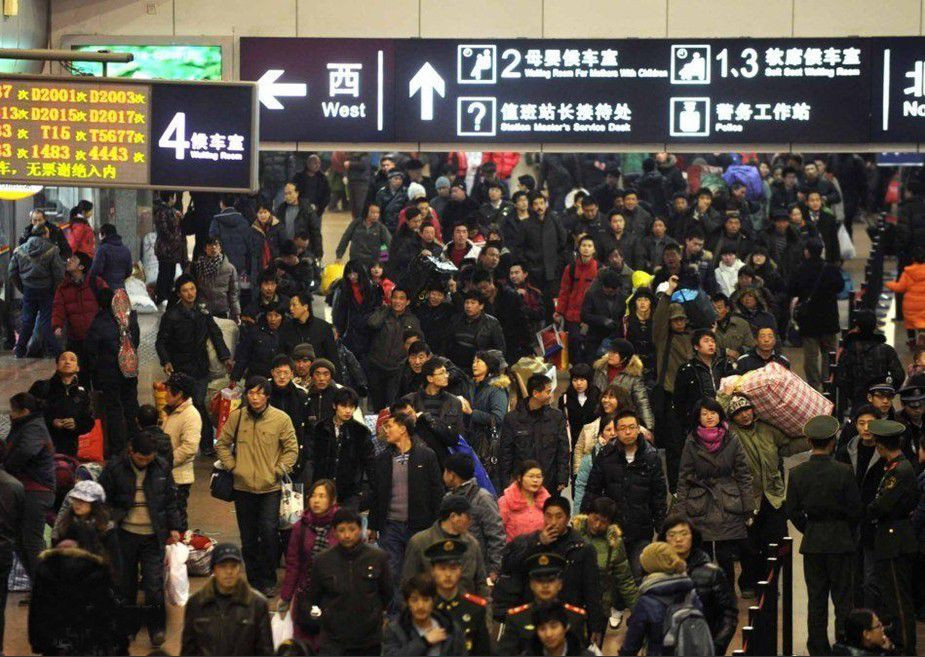
\includegraphics[width=0.6\linewidth]{chunyun}
    \caption{春运体现了中国人注重家庭团聚的主题}
\end{figure}

\subsubsection{春节经济}
春节是中国最重要和最具文化内涵的节日,更是推动产业经济和内需消费的重要内驱力。随着国民经济的快速增长,居民个人可支配收入不断提高,春节消费也由传统的置办年货发展为具有时代特色的贺岁作品、产品工艺、休闲娱乐等节日产品和服务。春节期间,人群、金融、物资、信息、艺术的大规模流动,带动了文化、商业、交通、旅游、电信、金融、餐饮各行各业全面繁荣,形成了独特的“春节经济”。
过年是人们一年消费的集中体现。随着新兴消费观念的不断涌现,春节已不仅仅是传统意义上的“过大年”,更是一个拉动市场经济动力的“快门”,人们开始从传统的节日忙碌转向新的庆贺潮流。“春节经济”为老百姓的生活注入了新的活力与生机。尽管大家不可能等到新年才有新衣穿、才有美食享用,但置办年货、孝敬长辈、关爱晚辈,依然是中华民族亘古不变的节日传统。





\subsubsection{国外影响}

\paragraph{各国年节}
随着中国综合国力的显著提升,中国文化的辐射领域也在不断扩大。春节的意义已经超过中国范畴,而具有世界影响。春节不是中国独有的节日,亚洲国家中,与中国一样过农历春节并有法定假期的包括越南、印尼、朝鲜、韩国、新加坡和马来西亚。另外,泰国、菲律宾和蒙古国也有过春节的传统。不过蒙古国过的是藏历春节,当地叫白月节,每年的节日起始日期要由喇嘛测算才能确定。

\paragraph{国外发展}
如今,春节已经走进全球近200个国家。据不完全统计,目前已有包括美国、加拿大、菲律宾、毛里求斯等在内近20个国家和地区,把中国春节定为整体或者所辖部分城市的法定节假日。2018年8月26日,美国加州多位力推认可农历新年法案的官员和华裔社区人士在旧金山召开发布会,欢庆法案正式生效。法案并未直接将农历新年定位为公众假日,但是鼓励学校和教育机构举办活动宣扬亚裔文化传统。

\paragraph{民族特色}
中国是个多民族的国家,各民族过新年的形式各有不同。古代的蒙古族,把春节叫做“白节”,正月叫白月,是吉祥如意的意思。藏族是过藏历年。回族、维吾尔族、哈萨克族等,是过“古尔邦节”。春节也是苗族、僮族、瑶族等的盛大节日。                                                        (简版)



\subsubsection{节令食品}

\paragraph{腊八粥}
“腊八节”这一天在中国部分地区有“喝腊八粥”的习俗(即是吃腊八粥)。喝腊八粥在中国已有千年历史,腊八粥又称“大家饭”。每逢腊八这一天,不论富人还是穷人,家家都要喝腊八粥。最早的腊八粥是用红小豆来煮,后经演变,加之地方特色,逐渐丰富多彩起来。
“腊八粥”又叫“七宝粥”“五味粥”,不仅清香甜美,而且能畅胃气,生津液,因而颇受人们喜食。随着时代的发展,花样越来越多的腊八粥已发展成具有地方风味的小吃。
\begin{figure}[htb]
    \centering
    \includegraphics[width=0.6\linewidth]{labazhou}
    \caption{腊八粥}
\end{figure}
\paragraph{年糕}
年糕属于农历新年的应时食品,有红、黄、白三色,象征金银。一种用黏性大的糯米或米粉蒸成的糕,在南方有过年吃年糕的习惯,甜甜的粘粘的年糕,象征新一年生活甜蜜蜜,步步高。
春节吃年糕,“义取年胜年,籍以祈岁稔。”寓意万事如意年年高。年糕的种类有:北方有白糕饦、黄米糕;江南有水磨年糕;西南有糯粑粑;台湾有红龟糕。北方年糕有蒸、炸二种,南方年糕除蒸、炸外,尚有片炒、汤煮诸法。 
\begin{figure}[htb]
    \centering
    \includegraphics[width=0.6\linewidth]{niangao}
    \caption{年糕}
\end{figure}
\paragraph{饺子}
饺子,古称“角子”,北方年夜饭有吃饺子的传统,但各地吃饺子的习俗亦不相同,有的地方除夕之夜吃饺子,有的地方初一吃饺子。三十晚上北方人不吃饺子,会觉得没有过年的气氛。北方一些山区还有初一到初五每天早上吃饺子的习俗。
\begin{figure}[htb]
    \centering
    \includegraphics[width=0.6\linewidth]{jiaozi}
    \caption{饺子}
\end{figure}
\paragraph{汤圆}
南方的元宵节庆食品叫做“汤圆”,别称“元宵”“汤团”“浮元子”,是中国传统小吃的代表之一,是由糯米粉等做的球状食品。一般有馅料,煮熟带汤食用。同时也是元宵节最具有特色的食物。用黑芝麻、猪油做馅、加入少许白砂糖,外面用糯米粉搓成圆形。因为这种糯米汤圆煮在锅里又浮又沉,所以它最早叫“浮元子”,后来有的地区把“浮元子”改称汤团。在江苏,上海等地,大年初一早晨都有吃汤圆的习俗。
\begin{figure}[htb]
    \centering
    \includegraphics[width=0.6\linewidth]{tangyuan}
    \caption{汤圆}
\end{figure}
\paragraph{春卷}
春卷也叫春饼,立春吃春饼是中国一种古老风俗。晋代已有“五芋盘”即“春盘”,是将春饼与菜同置一盘之内。
\begin{figure}[htb]
    \centering
    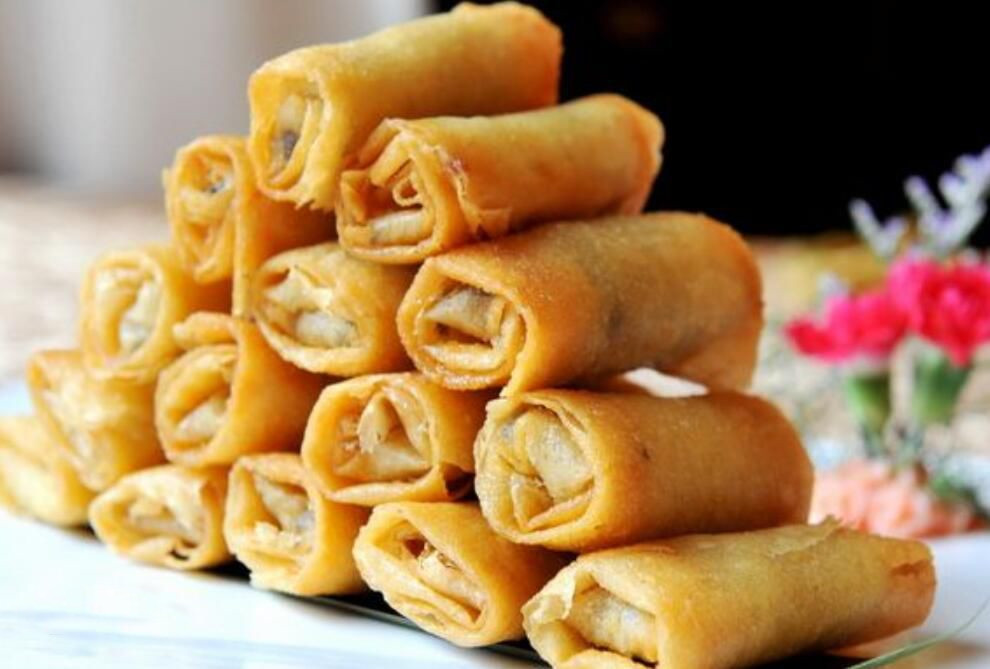
\includegraphics[width=0.6\linewidth]{chunjuan}
    \caption{春卷}
\end{figure}
\subsubsection{新年禁忌}
\begin{itemize}
\item 
小年各地的禁 忌各有不同。湖北部分地区,小年忌宰杀。河南有些地方忌讳捣蒜,认为小年捣蒜会把家里捣穷了。
\item
台湾称此日为“送神日”,禁忌舂米,据说能把风神捣下来,会给来年带来风灾。
\item 
小年后的几天,农村都会蒸馒头准备过年,但是不宜施舍给他人,因为这些馒头是要先用来祭祖祭天的。
\item 
还有,灶糖不宜多吃。过小年要吃灶糖,糖尿病患者宜少吃。灶糖是一种麦芽糖,粘性很大,把它抽为长条型的糖棍称为“关东糖”,拉制成扁圆型就叫做“糖瓜”。
\end{itemize}